\documentclass{article}

% if you need to pass options to natbib, use, e.g.:
% \PassOptionsToPackage{numbers, compress}{natbib}
% before loading neurips_2019

% ready for submission
\usepackage{neurips_2019}

% to compile a preprint version, e.g., for submission to arXiv, add add the
% [preprint] option:
%\usepackage[preprint]{neurips_2019}

% to compile a camera-ready version, add the [final] option, e.g.:
% \usepackage[]{neurips_2019}

% to avoid loading the natbib package, add option nonatbib:
% \usepackage[nonatbib]{neurips_2019}

\usepackage[utf8]{inputenc} % allow utf-8 input
\usepackage[T1]{fontenc}    % use 8-bit T1 fonts
\usepackage{hyperref}       % hyperlinks
\usepackage{url}            % simple URL typesetting
\usepackage{booktabs}       % professional-quality tables
\usepackage{amsfonts}       % blackboard math symbols
\usepackage{nicefrac}       % compact symbols for 1/2, etc.
\usepackage{microtype}      % microtypography

%--------------------------------------------------------------------------------------------------------------------------------% 

\RequirePackage{mathrsfs, amsthm, amsmath, amsfonts, amssymb, mathtools}%
\usepackage[titletoc,title]{appendix}%
\usepackage{dsfont}%
\usepackage{caption} % 
\usepackage{subcaption}
\usepackage{float}%
\usepackage{graphicx, color}% 
\usepackage{bm}%bold equations

%% formatting appendices
\usepackage{etoolbox}
\usepackage{natbib}
\patchcmd{\appendices}{\quad}{. }{}{}

%% tables
\usepackage{pgfplots}%
\usepackage{booktabs,multirow,array,multicol}
\newcommand{\otoprule}{\midrule[\heavyrulewidth]}

%% algorithms
\usepackage[linesnumbered,ruled,vlined]{algorithm2e}
\usepackage{enumitem}

\setlist[itemize]{leftmargin=4.5mm}

\usepackage{accents}
\usepackage{datenumber}
\usepackage{wrapfig}

\newcommand{\rev}[1]{{\color{blue} #1}}
\newcommand{\ar}[1]{{\color{red} #1}}
\newcommand{\rf}[1]{{\color{green} #1}}

%% sections
\newtheorem{theorem}{Theorem}
\newtheorem{corollary}{Corollary}
\newtheorem{lemma}{Lemma}
\newtheorem{fact}{Fact}
\newtheorem{proposition}{Proposition}
\newtheorem{definition}{Definition}%[section]
\newtheorem*{notation}{Notation}%[section]
\newtheorem{discus}{Discussion}%[section]
\newtheorem{remark}{Remark}%[section]
\newtheorem{example}{Example}%[section]
\newtheorem{exs}{Examples}%[section]
\newtheorem{ca}{Cas}
\newtheorem{remarks}{Remarks}%[section]
\newtheorem{assumption}{Assumption}{\bf}{\rm}%

% math macros
\newcommand{\bigO}{\mathcal{O}}
\newcommand{\inr}[1]{\langle #1 \rangle}
\newcommand{\ind}[1]{{\mathds{1}}_{{#1}}}%
\newcommand{\norm}[1]{\|#1\|}
\newcommand{\R}{{\mathbb{R}}}
\newcommand{\E}{\mathds{E}}
\newcommand{\bcdot}{\raisebox{-0.80ex}{\scalebox{1.8}{$\cdot$}}}
\newcommand{\varsig}{\raisebox{-0.15ex}{\scalebox{1.30}{$\varsigma$}}}
\newcommand*{\dt}[1]{\accentset{\mbox{\large\bfseries .}}{#1}}

%% math operators
\DeclareMathOperator*{\argmin}{\arg\!\min}
\DeclareMathOperator*{\argmax}{\arg\!\max}
%--------------------------------------------------------------------------------------------------------------------------------%

\title{Screening Sinkhorn Algorithm for Regularized Optimal Transport}

\begin{document}

\author{%
Mokhtar Z. Alaya \\
LITIS EA4108\\
University of Rouen\\
\texttt{mokhtarzahdi.alaya@gmail.com} 
\And
Maxime Bérar\\
LITIS EA4108\\
University of Rouen\\
\texttt{maxime.berar@univ-rouen.fr} \\
\And
Gilles Gasso \\
LITIS EA4108\\
INSA, University of Rouen\\
\texttt{gilles.gasso@insa-rouen.fr} 
\And
Alain Rakotomamonjy\\
LITIS EA4108 \\
University of Rouen\\
and Criteo AI Lab, Criteo Paris \\
\texttt{alain.rakoto@insa-rouen.fr} \\
}

\maketitle

\begin{abstract}
We introduce in this paper a novel strategy for efficiently approximate the Sinkhorn distance between two discrete measures. After identifying neglectible components
of the dual solution of the regularized Sinkhorn problem, we propose to screen those components by directly setting them at that value before entering the Sinkhorn problem. This allows us to solve a smaller Sinkhorn problem while ensuring approximation with provable guarantees.
More formally, the approach is based on a reformulation of \emph{dual of Sinkhorn divergence problem} and on the KKT optimality conditions of this problem, which enable identification of dual components to be screened.
This new analysis leads to the \emph{Screenkhorn} algorithm.
We illustrate the efficiency of Screenkhorn on complex tasks such as dimensionality reduction or domain adaptation involving regularized optimal transport.
\end{abstract}

%!TEX root = main.tex

\section{Introduction} % (fold)
\label{sec:introduction}

Computing OT distances between pairs of probability measures or histograms, such as the earth mover's distance~\citep{werman1985,Rubner2000} and Monge-Kantorovich or Wasserstein distance~\citep{villani09optimal}, are currently generating an increasing attraction in different machine learning tasks~\citep{pmlr-v32-solomon14,kusnerb2015,pmlr-v70-arjovsky17a,ho2017}, statistics~\citep{frogner2015nips,panaretos2016,ebert2017ConstructionON,bigot2017,flamary2018WDA}, and computer vision~\citep{bonnel2011,Rubner2000,solomon2015}, among other applications~\citep{klouri17,peyre2019COTnowpublisher}.
In many of these problems, OT exploits the geometric features of the objects at hand in the underlying spaces to be leveraged in comparing probability measures.
This effectively leads to improve performance of methods that are oblivious to the geometry, for example the chi-squared distances or the Kullback-Leibler divergence.
Unfortunately, this advantage comes at the price of an enormous computational cost of solving the OT problem, that can be prohibitive in large scale applications.
For instance, the OT between two histograms with supports of equal size $n$ can be formulated as a linear programming problem that requires generally super $\bigO(n^3)$~\citep{pele2009} arithmetic operations, which is problematic when $n$ is larger than $10^3.$

A remedy to the heavy computation burden of OT lies in a prevalent approach referred as regularized OT~\citep{cuturinips13} and operates by adding an entropic regularization penalty to the original problem.  
Such a regularization guarantees a unique solution, since the objective function is strongly convex, and a greater computational stability.
Furthermore,~\citet{cuturinips13} proposed the so-called {dual of Sinkhorn divergence} as the dual of the entropic problem and noticed that finding the dual solution was equivalent to finding two diagonal matrices that made a full matrix bistochastic.
Therefore, the OT can be solved efficiently with celebrated matrix scaling algorithms, such as Sinkhorn's fixed point iteration method~\citep{sinkhorn1967,knight2008,kalantari2008}. 

Sinkhorn scaling for computing OT distances is a well studied problem in many recent works. 
The main idea is to improve the matrix-vector operations that are the computational bottleneck of Sinkhorn’s algorithm. 
\citet{altschulernips17} proposed a greedy version of Sinkhorn, called Greenkhorn algorithm, allowing to select columns and rows to be updated that most violate the constraints.                   
Another approach based on low-rank approximation of the cost matrix using Nystrom method induces the Nys-Sink algorithm~\citep{altschuler2018Nystrom}. 
Other classical optimization algorithms have been considered to approximate the OT, for instance accelerated gradient descent~\citep{xie2018proxpointOT,dvurechensky18aICML,lin2019}, quasi Newton methods~\citep{blondel2018ICML,cuturi2016SIAM} and stochastic gradient descent~\citep{genevay2016stochOT,khalilabid2018}. 

{In this paper, we propose a novel technique for accelerating the Sinkhorn algorithm when computing regularized OT distance between discrete measures. Our idea
is strongly related to a screening strategy when solving a \emph{Lasso}
problem in sparse supervised learning \citep{Ghaoui2010SafeFE}. Based on the fact
that a  transport plan resulting from an OT problem is sparse or presents a large
number of neglectable values \citep{blondel2018ICML}, our objective is to identify the  dual variables of an approximate Sinkhorn problem, that are smaller than a predefined threshold, and thus that can be safely removed before optimization.  
Within this global context, our contributions are the following :
\begin{itemize}
	  \setlength\itemsep{-0.1cm}
	
	\item From a methodological point of view, we propose a reformulation the dual of the Sinkhorn divergence problem by imposing variables to be larger than a threshold.
	This formulation allows us to introduce sufficient conditions, computable beforehand, for a variable to be strictly satisfied its constraint, leading then to
	a ``screened'' version of the dual of Sinkhorn divergence. 
	\item We provide some theoretical analysis of the solution of the ``screened''  Sinkhorn divergence, showing that its objective value and the marginal constraint satisfaction are properly controlled 	as the number of screened variables decreases.
	\item From an algorithmic standpoint, we use a constrained LBFGS algorithm \citep{nocedal1980,byrd1995L-BFGS-B} but provide a careful analysis of the lower bound and upper bound of the dual	variables, resulting in a well-posed and efficient algorithm denoted as \emph{Screenkhorn}.
	\item Our empirical analysis depicts how the approach behaves in a simple Sinkhorn divergence computation context. When considered in  complex machine learning
	pipelines, we show that \emph{Screenkhorn} can lead to strong gain in efficiency
	while not compromising on accuracy.
\end{itemize}}
%	
%
%These constraints are defined through a convex set which depends on two parameters acting like threshold and scaling factor.
%We prove that dual solution of this reformulation guarantees the existence of two active indices sets for the potential variables.
%Furthermore, the active sets are both directly linked to a priori fixed number budget of points from the supports of the given discrete measures.
%We then restrict the constraints feasibility by taking into account the properties providing by the active sets to get a ``screened'' version of the dual of Sinkhorn divergence. 
%Screenkhorn algorithm developed in this paper consists of two steps; the first one is an initialization step devoted to determine the active sets while the second is a constrained box-constrained L-BFGS-B solver, a limited-memory quasi-Newton algorithm~\cite{nocedal1980,byrd1995L-BFGS-B} that relies on an estimation of the inverse of the Hessian based on gradients differences. 
%L-BFGS-B algorithm was adapted to the OT setting via the dual of Sinkhorn divergence in ~\cite{cuturi2016SIAM,blondel2018ICML}.}

The remainder of the paper is organized as follow. In Section~\ref{sec:regularized_discrete_ot} we briefly review the basic setup of regularized discrete OT. 
Section~\ref{sec:screened_dual_of_sinkhorn_divergence} contains our main contribution, that is, the Screenkhorn algorithm. 
Section~\ref{sec:analysis_of_marginal_violations} devotes to theoretical guarantees for marginal violations of Screenkhorn. 
In Section~\ref{sec:numerical_experiments} we present numerical results for the proposed algorithm, compared with the state-of-art Sinkhorn algorithm as implemented in~\cite{flamary2017pot}. 
The proofs of theoretical results are postponed to the supplementary material.

\emph{Notation.} For any positive matrix $T \in \R^{n\times m}$, we define its negative entropy as $H(T) = -\sum_{i,j} T_{ij} \log(T_{ij}).$
Let $r(T) = T\mathbf 1_m \in \R^n$ and $c(T) = T^\top\mathbf 1_n \in \R^m$ denote the rows and columns sums of $T$ respectively. The coordinates $r_i(T)$ and $c_j(T)$ denote the $i$-th row sum and the $j$-th column sum of $T$, respectively.
The scalar product between two matrices denotes the usual inner product, that is $\inr{T, W} = \text{tr}(T^\top W) = \sum_{i,j}T_{ij}W_{ij},$ where $T^\top$ is the transpose of $T$. 
We write $\mathbf{1}$ (resp. $\mathbf{0}$) the vector having all coordinates equal to one (resp. zero).
$\Delta(w)$ denotes the diag operator, such that if $w \in \R^n$, then $\Delta(w) = \text{diag}(w_1, \ldots, w_n)\in \R^{n\times n}$.
For a set of indices $L=\{i_1, \ldots, i_k\} \subseteq \{1, \ldots, n\}$ satisfying $i_1 < \cdots <i_k,$ we denote the complementary set of $L$ by $L^\complement = \{1, \ldots, n\} \backslash L$. We also denote $|L|$ the cardinality of $L$.
Given a vector $w \in \R^n$, we denote $w_L= (w_{i_1}, \ldots, w_{i_k})^\top \in \R^k$ and its complementary $w_{L^\complement} \in \R^{n- k}$.  The notation is similar for matrices; given another subset of indices $S = \{j_1, \ldots, j_l\} \subseteq \{1, \ldots, m\}$ with $j_1 < \cdots <j_l,$ and a matrix $T\in \R^{n\times m}$, we use $T_{(L,S)}$, to denote the submatrix of $T$, namely the rows and columns of $T_{(L,S)}$ are indexed by $L$ and $S$ respectively.
When applied to matrices and vectors,  $\odot$ and $\oslash$ (Hadamard product and division) and exponential notations refer to elementwise operators.
Given two real numbers $a$ and $b$, we write $a\vee b = \max(a,b)$ and $a\wedge b = \min(a,b).$

% section introduction (end)
%!TEX root = main.tex

\section{Regularized discrete OT} % (fold)
\label{sec:regularized_discrete_ot}

We briefly expose in this section the setup of OT between two discrete measures. We then consider the case when those distributions are only available through a finite number of samples, that is $\mu = \sum_{i=1}^n \mu_i \delta_{x_i} \in \Sigma_n$ and $\nu = \sum_{j=1}^m \nu_i \delta_{y_j} \in \Sigma_m$, where $\Sigma_n$ is the probability simplex with $n$ bins, namely the set of probability vectors in $\R_+^n$, i.e., $\Sigma_n = \{w \in \R_+^n: \sum_{i=1}^n w_i = 1\}.$
We denote their probabilistic couplings set as $\Pi(\mu, \nu) = \{P \in \R_+^{n\times m}, P\mathbf{1}_m = \mu, P^\top \mathbf{1}_n = \nu\}.$ 
\paragraph{Sinkhorn divergence.}

Computing OT distance between the two discrete measures $\mu$ and $\nu$  amounts to solving a linear problem~\citep{kantorovich1942} given by
\begin{equation*}
  \label{monge-kantorovich}
  \mathcal{S}(\mu, \nu) =  \min_{P\in \Pi(\mu, \nu)} \inr{C, P},
\end{equation*}
where $P= (P_{ij}) \in \R^{n\times m}$ is called the transportation plan, namely each entry $P_{ij}$ represents the fraction of mass moving from $x_i$ to $y_j$, and $C= (C_{ij}) \in \R^{n\times m}$ is a cost matrix comprised of nonnegative elements and related to the energy needed to move a probability mass from $x_i$ to $y_j$. 
The entropic regularization of OT distances~\citep{cuturinips13} relies on the addition of a penalty term as follows:
\begin{equation}
\label{sinkhorn-primal}
  \mathcal{S}_\eta(\mu, \nu) =  \min_{P\in \Pi(\mu, \nu)} \{\inr{C, P} - \eta H(P)\},
\end{equation}
where $\eta > 0$ is a regularization parameter. We refer to $\mathcal{S}_\eta(\mu, \nu) $ as the \emph{Sinkhorn divergence}~\citep{cuturinips13}.

\paragraph{Dual of Sinkhorn divergence.}

Below we provide the derivation of the dual problem for the regularized OT problem~\eqref{sinkhorn-primal}. Towards this end, we begin with writing its Lagrangian dual function:
\begin{equation*}
  \mathscr{L}(P,w, z) = \inr{C,P} + \eta \inr{\log P, P} + \inr{w, P\mathbf{1}_m - \mu} + \inr{z,P^\top \mathbf{1}_n - \nu}.
\end{equation*}
The dual of Sinkhorn divergence can be derived by solving $\min_{P \in \R_+^{n\times m}}\mathscr{L}(P,w, z)$. It is easy to check that objective function $P\mapsto \mathscr{L}(P,w, z)$ is strongly convex and differentiable. Hence, one can solve the latter minimum by setting $\nabla_P \mathscr{L}(P,w, z)$ to $\mathbf{0}_{n\times m}$. Therefore, we get $  P^\star_{ij} = \exp\big(- \frac{1}{\eta} (w_i + z_j + C_{ij}) - 1\big), 
$ for all $i=1, \ldots, n$ and $j=1, \ldots, m$. Plugging this solution,  and setting the change of variables $u = -w/\eta - 1/2$ and $v = - z/\eta - 1/2$, the dual problem is given by
\begin{equation}
\label{sinkhorn-dual}
\min_{u \in \R^n, v\in\R^m}\big\{\Psi(u,v):= \mathbf{1}_n^\top B(u,v)\mathbf{1}_m - \inr{u, \mu} - \inr{v, \nu} \big\},
\end{equation}
where $B(u,v) := \Delta(e^{u}) K \Delta(e^{v})$ and $K := e^{-C/\eta}$ stands for the Gibbs kernel associated to the cost matrix $C$. 
We refer to problem~\eqref{sinkhorn-dual} as the \emph{dual of Sinkhorn divergence}. Then, the optimal solution $P^\star$ of the primal problem~\eqref{sinkhorn-primal} takes the form $P^\star = \Delta(e^{u^\star}) K \Delta(e^{v^\star})$
where the couple $(u^\star, v^\star)$ satisfies:
\begin{align*}
\label{sinkhorn-dual}
  (u^\star, v^\star) &= \argmin_{u \in \R^{n}, v\in \R^m} \{\Psi(u,v)\}.
\end{align*}
Note that the matrices $\Delta(e^{u^\star})$ and $\Delta(e^{v^\star})$ are unique up to a constant factor~\citep{sinkhorn1967}. Moreover, $P^\star$ can be solved efficiently by iterative Bregman projections~\citep{benamou2015IterativeBP} referred to as Sinkhorn iterations, and the method is referred to as \textsc{Sinkhorn} algorithm which, recently, has been proven to achieve a near-$\bigO(n^2)$ complexity~\citep{altschulernips17}.

% section regularized_discrete_ot (end)
%!TEX root = main.tex

\section{Screened dual of Sinkhorn divergence} % (fold)
\label{sec:screened_dual_of_sinkhorn_divergence}

\begin{wrapfigure}{o}{0.44\textwidth}
\vspace{-15pt}
\centering
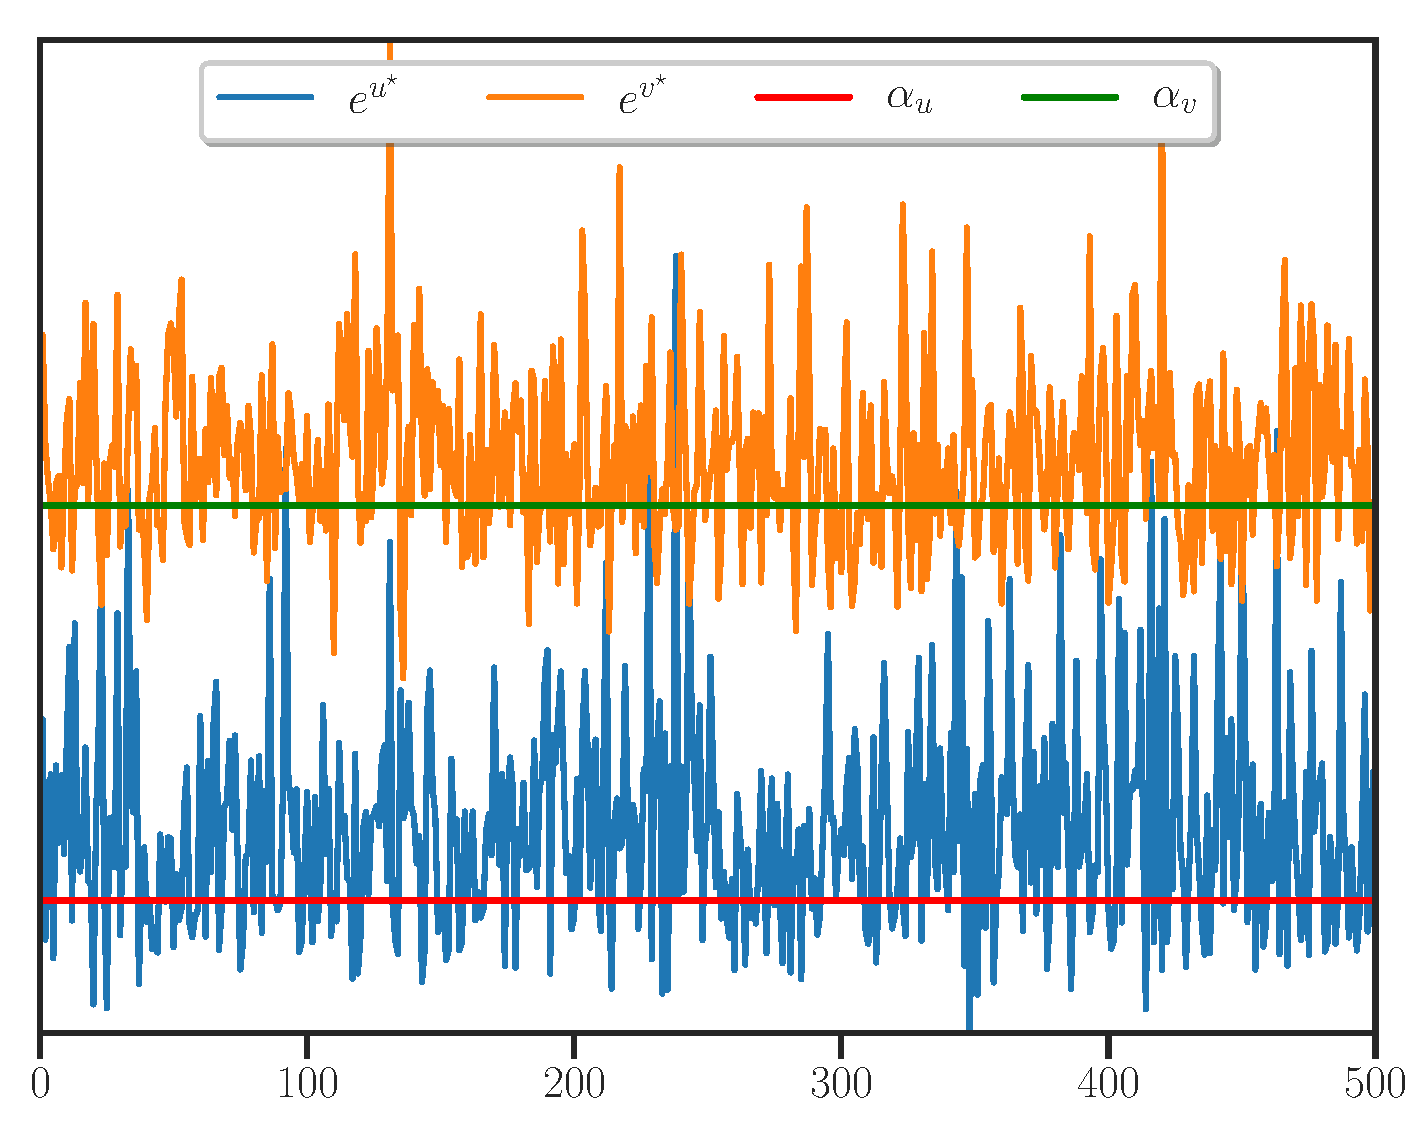
\includegraphics[width=0.45\textwidth]{./figs/motivations.pdf}
\caption{Plots of $(e^{u^\star}, e^{v^\star})$ pair solution of dual of Sinkhorn divergence~\ref{sinkhorn-dual}.}
\label{fig:motivations}
\vspace{-11pt}
\end{wrapfigure}

\paragraph{Motivation.} 

The key idea of our approach is motivated by the so-called \emph{static screening test}~\citep{Ghaoui2010SafeFE} in supervised learning, which is a method able to quickly identify inactive features, i.e., features that have zero components in the solution vector. 
Then, these inactive features can be removed from the optimization problem to reduce its scale.
Before diving into detailed algorithmic analysis, let's us present a brief illustration of how we adapt static screening test to the dual of Sinkhorn divergence.
Towards this end, we define the convex set $\mathcal{C}^r_{\alpha} \subseteq \R^r$, for $r\in \mathbb N$ and $\alpha >0$, by $\mathcal{C}^r_{\alpha} = \{w\in \R^{r}: \min_{1\leq i\leq r} e^{w_i} \geq \alpha\}$.
In Figure~\ref{fig:motivations}, we plot $(e^{u^\star}, e^{v^\star})$ solution of dual of Sinkhorn divergence~(\ref{sinkhorn-dual}) in the particular case of: $n=m=500, \eta=0.1, \mu = \nu = \frac 1n \mathbf 1_n$ and the cost matrix $C$ corresponds the pairwise euclidean distance, i.e., $C_{ij} = \norm{x_i - y_j}_2$. 
We also plot two lines corresponding to $e^{u^\star} \equiv \alpha_u$ and $e^{v^\star} \equiv \alpha_v$ for some $\alpha_u>0$ and $\alpha_v >0$, playing the role of thresholds to select indices to be discard from the optimization procedure.

\paragraph{Static screening test.} The core of the static screening test developed in this paper aims at locating two subsets of indices $(I, J)$ in $\{1, \ldots, n\}\times\{1, \ldots, m\}$ satisfying: $e^{u_i}\geq \alpha_u, \text{ and } e^{v_j}\geq \alpha_v, \text{ for all } (i,j) \in I \times J$ and 
$e^{u_{i'}} = \alpha_u, \text{ and } e^{v_{j'}} = \alpha_v, \text{ for all } (i',j') \in I^\complement \times J^\complement$, namely $(u,v) \in \mathcal{C}^n_{\alpha_u}\times \mathcal{C}^m_{\alpha_v}$.
The sets $I$ and $J$ are called active sets, we further emphasize that they are determined in an initialization step in the proposed algorithm before running the L-BFGS-B solver.
Consequently, we can work on a "screened" dual of Sinkhorn divergence by considering variables that belong only to $\R^{|I|} \times \R^{|J|}$ in order to reduce the computational cost.

In the following, the parameters $\alpha_u = \varepsilon \kappa^{-1}$ and $\alpha_v = \varepsilon \kappa$ where $\varepsilon > 0$ and $\kappa > 0$ are fixed numeric constants to be given later. 
Our screening test relies on a new formulation of problem~\eqref{sinkhorn-dual}, that we refer as to \emph{approximate dual of Sinkhorn divergence}, defined by:

\begin{equation} 
\label{screen-sinkhorn}
\min_{u \in \mathcal{C}^n_{\frac \varepsilon \kappa}, v\in \mathcal{C}^m_{\varepsilon\kappa}} \big\{\Psi_{\kappa}(u,v):= \mathbf{1}_n^\top B(u,v)\mathbf{1}_m - \inr{\kappa u, \mu} - \inr{\frac v\kappa, \nu} \big\},
\end{equation}
The $\kappa$-parameter plays a role of scaling factor, allowing to get a closed order of the potential components $e^u$ and $e^v$, while the $\varepsilon$-parameter acts like a threshold for these components.
Note that the approximate dual of Sinkhorn divergence coincides with the dual of Sinkhorn divergence~\eqref{sinkhorn-dual} in the setting of $\varepsilon=0$ and $\kappa=1$.
As explained above, our static screening test is based on constructing two {active sets} denoted $I_{\varepsilon, \kappa}$ and $J_{\varepsilon, \kappa}$ throughout the dual problem of~\eqref{screen-sinkhorn} as follows: 

\begin{lemma}
\label{lemma_actives_sets}
Let $(u^{*}, v^{*})$ be an optimal solution of problem~\eqref{screen-sinkhorn}. 
Define
\begin{equation}
\label{I_epsilon_kappa_J_epsilon_kappa}
I_{\varepsilon,\kappa} = \big\{i=1, \ldots, n: \mu_i \geq \frac {\varepsilon^2} \kappa^{} r_i(K)\big\}, J_{\varepsilon,\kappa} = \big\{j=1, \ldots, m: \nu_j \geq \kappa{\varepsilon^2}{} c_j(K)\big\}
\end{equation}
Then one has $e^{u^{*}_i} = \varepsilon\kappa^{-1}$ and $e^{v^{*}_j} = \varepsilon\kappa$ for all $i \in I^\complement_{\varepsilon,\kappa} $ and $j\in J^\complement_{\varepsilon,\kappa} .$
\end{lemma}

Proof of Lemma~\ref{I_epsilon_kappa_J_epsilon_kappa} is postponed to the supplementary material. It is worth to note that first order conditions applied to $(u^{*}, v^{*})$ ensure that if $e^{u^{*}_i} > \varepsilon\kappa^{-1}$ then $e^{u^{*}_i} (Ke^{v^{*}})_i =  \kappa\mu_i$ and if $e^{v^{*}_j} > \varepsilon\kappa$ then $e^{v^{*}_j} (K^\top e^{u^{*}})_j =  \kappa^{-1}\nu_j$, that correspond to the Sinkhorn marginal conditions~\citep{peyre2019COTnowpublisher} up to the scaling factor $\kappa$. 

\paragraph{Screening with a fixed number budget of points.}

Recall that the approximate dual of Sinkhorn divergence is defined with respect to $\varepsilon$ and $\kappa$, where its values depend on a priori \emph{fixed number budget of points} from the supports of $\mu$ and $\nu$.
In the sequel, we denote by $n_b \in\{1, \ldots, n\}$ and $m_b\in\{1, \ldots, m\}$ the number budget of points to be given for resolving problem~\eqref{screen-sinkhorn}. More precisely, we change the domain of the objective function $\Psi_\kappa$ from $\R^n \times \R^m$ to $\R^{n_b} \times \R^{m_b}$.

\begin{wrapfigure}{o}{0.44\textwidth}
\vspace{-18pt}
\centering
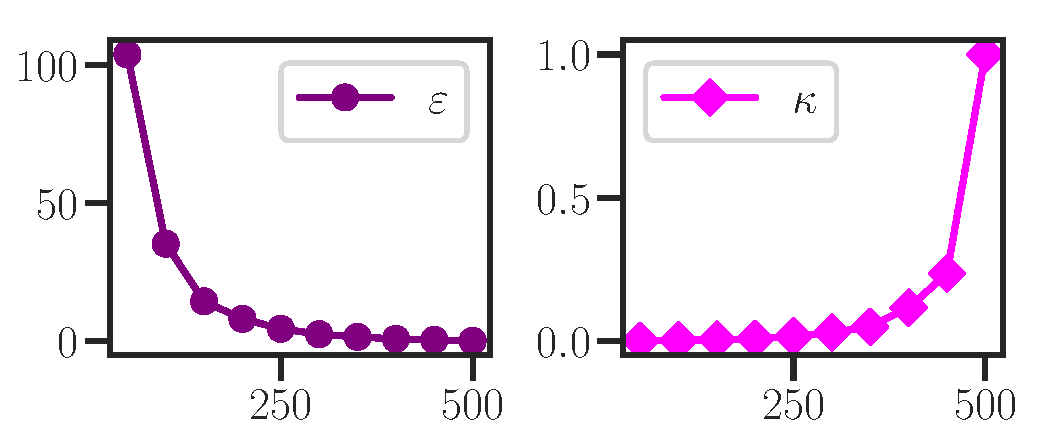
\includegraphics[width=0.46\textwidth]{./figs/kappa_epsilon.pdf}
\caption{Plots of $\varepsilon$ and $\kappa$ as a function of budget of points for a screening test with $n_b=m_b$ and the parameters $\mu, \nu, \eta, C$ are set as in Figure~\eqref{fig:motivations}. As it can be seen, $(\varepsilon, \kappa)$ tends to $(0,1)$ as $(n_b,m_b)$ tends to $(n,m)$.}
\label{fig:kappa_epsilon}
\vspace{-15pt}
\end{wrapfigure}

In this spirit, let us define $\xi \in \R^n$ and $\zeta \in \R^m$ to be the ordered decreasing vectors of $\mu \oslash r(K)$ and $\nu \oslash c(K)$ respectively, that is $\xi_1 \geq \xi_2 \geq \cdots \geq \xi_n$ and $\zeta_1 \geq \zeta_2 \geq \cdots \geq \zeta_m$.
To keep only $n_b$-budget and $m_b$-budget of points, the parameters $\kappa$ and $\varepsilon$ satisfy ${\varepsilon^2}\kappa^{-1} = \xi_{n_b}$ and $\varepsilon^2\kappa = \zeta_{m_b}$. Hence 
\begin{equation}
\label{epsilon_kappa}
 \varepsilon = (\xi_{n_b}\zeta_{m_b})^{1/4} \text{ and } \kappa = \sqrt{\frac{\zeta_{m_b}}{\xi_{n_b}}}.
\end{equation}
Note that in one hand we have $|I_{\varepsilon, \kappa}| = n_b$ and $|J_{\varepsilon, \kappa}| = m_b$ by construction. On the other hand, when $(n_b,m_b)$ tends to the full number budget of points $(n,m)$, the couple parameters $(\varepsilon, \kappa)$ converges to $(0,1)$. 
In Figure~\ref{fig:kappa_epsilon}, we plot these convergences, and hence in this case the approximate dual in problem \eqref{screen-sinkhorn} corresponds to the dual of Sinkhorn divergence~\eqref{sinkhorn-dual}.

Using the previous analysis, any solution $(u^*, v^*)$ of problem~\eqref{screen-sinkhorn} satisfies $e^{u^*_i} \geq \varepsilon\kappa^{-1}$ and $e^{v^*_j} \geq \varepsilon\kappa$ for all $(i,j) \in (I_{\varepsilon,\kappa}\times J_{\varepsilon,\kappa}),$ and $e^{u^*_i} = \varepsilon\kappa^{-1}$ and $e^{v^*_j} = \varepsilon\kappa$ for all $(i,j) \in (I^\complement_{\varepsilon,\kappa}\times J^\complement_{\varepsilon,\kappa})$.
Basing on that facts we restrict the constraints feasibility $\mathcal{C}^n_{\frac \varepsilon \kappa} \cap \mathcal{C}^m_{\varepsilon\kappa}$ to the screened domain defined by $\mathcal{U}_{\text{sc}} \cap \mathcal{V}_{\text{sc}}$ where 
\begin{equation*}
\mathcal{U}_{\text{sc}} = \{u \in \R^{n_b}: e^{u_{I_{\varepsilon,\kappa}}} \succeq \frac \varepsilon\kappa\mathbf 1_{n_b}\} \text{ and } \mathcal{V}_{\text{sc}} =\{v\in\R^{m_b}: e^{v_{J_{\varepsilon,\kappa}}} \succeq \varepsilon\kappa \mathbf{1}_{m_b}\}.%, \text{ and } e^{u_{I^\complement_{\varepsilon,\kappa}}} = \frac\varepsilon\kappa\mathbf 1_{n - n_b}\},
\end{equation*}
% and 
% \begin{equation*}
% 	\mathcal{V}_{\text{sc}} =\{v\in\R^m: e^{v_{J_{\varepsilon,\kappa}}} \succeq \varepsilon\kappa \mathbf{1}_{m_b}\}. %, \text{ and } e^{v_{J^\complement_{\varepsilon,\kappa}}} = \varepsilon\kappa \mathbf 1_{m- m_b}\}.
% \end{equation*}
where the vector comparison $\succeq$ has to be understood elementwise.
Now, we are ready to define the \emph{screened dual of Sinkhorn divergence} as
\begin{align}
\label{screen-sinkhorn_second_def}
\min_{u \in \mathcal{U}_{\text{sc}}, v \in \mathcal{V}_{\text{sc}}}\{\Psi_{\varepsilon, \kappa}(u,v)\}
\end{align}
where 
\begin{align*} 
\Psi_{\varepsilon,\kappa}(u, v) &= (e^{u_{I_{\varepsilon,\kappa}}})^\top K_{(I_{\varepsilon,\kappa}, J_{\varepsilon,\kappa})} e^{v_{J_{\varepsilon,\kappa}}} + 
\varepsilon \kappa (e^{u_{I_{\varepsilon,\kappa}}})^\top K_{(I_{\varepsilon,\kappa}, J^\complement_{\varepsilon,\kappa})}\mathbf 1_{m_b} + \varepsilon \kappa^{-1} \mathbf 1_{n_b}^\top K_{(I^\complement_{\varepsilon,\kappa}, J_{\varepsilon,\kappa})}e^{v_{J_{\varepsilon,\kappa}}}\\
&\qquad - \kappa \mu_{I_{\varepsilon,\kappa}}^\top u_{I_{\varepsilon,\kappa}} - \kappa^{-1} \nu_{J_{\varepsilon,\kappa}}^\top v_{J_{\varepsilon,\kappa}} + \Xi
\end{align*}
with $\Xi = \varepsilon^2 \sum_{i \in I^\complement_{\varepsilon,\kappa}, j \in J^\complement_{\varepsilon,\kappa}} K_{ij} -\kappa \log(\varepsilon\kappa^{-1})\sum_{i \in I^\complement_{\varepsilon,\kappa}}\mu_i - \kappa^{-1} \log(\varepsilon\kappa)\sum_{j\in J^\complement_{\varepsilon,\kappa}} \nu_j$.

Pseudocode of our proposed algorithm is shown in Algorithm~\ref{screenkhorn}. %~\cite{nocedal1980,nocedal2006numerical}
It is worth to note that Screenkhorn algorithm uses only the restricted parts $K_{(I_{\varepsilon,\kappa}, J_{\varepsilon,\kappa})},$ $K_{(I_{\varepsilon,\kappa}, J^\complement_{\varepsilon,\kappa})},$ and $K_{(I^\complement_{\varepsilon,\kappa}, J_{\varepsilon,\kappa})}$ of the Gibbs kernel $K$ for calculating the objective function $\Psi_{\varepsilon, \kappa}$ and its gradient, in contrast to Sinkhorn algorithm which performs alternating updates of all rows and columns of $K.$
Furthermore, Screenkhorn consists of two steps: the first one is an initialization providing the active sets $I_{\varepsilon,\kappa}$, $J_{\varepsilon,\kappa}$. 
The second is a constrained L-BFGS-B for the stacked variable $\theta=(u_{I_{\varepsilon,\kappa}},v_{J_{\varepsilon,\kappa}}).$ 
L-BFGS-B handles box constraints on variables, and it becomes more efficient when these box bounds are carefully determined for problem~\eqref{screen-sinkhorn_second_def}. 
The following proposition (proof in supplementary material) expresses these bounds that are pre-calculated in the initialization step of \emph{Screenkhorn}.
\begin{proposition}
\label{prop:bounds_of_usc_and_vsc}
Let $(u^{\text{sc}}, v^{\text{sc}})$ be an optimal pair solution of problem~\eqref{screen-sinkhorn_second_def} and $K_{\min} = \min\limits_{i\in I_{\varepsilon,\kappa},j \in J_{\varepsilon,\kappa}}K_{ij}$. Then,
one has
\begin{equation}
\label{bound_on_u}
\frac \varepsilon\kappa \vee \frac{\min_{i \in I_{\varepsilon,\kappa}}\mu_i}{\varepsilon (m- m_b) + \varepsilon \vee \frac{\max_{j\in J_{\varepsilon,\kappa}} \nu_j}{n\varepsilon\kappa K_{\min}} m_b} \leq e^{u^{\text{sc}}_i} \leq \frac \varepsilon\kappa\vee \frac{\max_{i \in I_{\varepsilon,\kappa}} \mu_i}{m\varepsilon K_{\min}},
\end{equation}
and
\begin{equation}
\label{bound_on_v}
\varepsilon\kappa \vee \frac{\min_{j \in J_{\varepsilon,\kappa}}\nu_j}{\varepsilon(n- n_b) + \varepsilon \vee \frac{\kappa\max_{i\in I_{\varepsilon,\kappa}} \mu_i}{m\varepsilon K_{\min} } n_b} \leq e^{v^{\text{sc}}_j} \leq \varepsilon\kappa \vee \frac{\max_{j \in J_{\varepsilon,\kappa}} \nu_j}{n\varepsilon K_{\min} }
\end{equation}
for all $i\in I_{\varepsilon,\kappa}$ and $j\in J_{\varepsilon,\kappa}$.
\end{proposition}
\LinesNotNumbered
\begin{algorithm}[htbp]
\SetNlSty{textbf}{}{.}
\DontPrintSemicolon
\caption{Screenkhorn$(C,\eta,\mu,\nu,n_b,m_b)$}
\label{screenkhorn}

\textbf{Step 1:} \textcolor{black}{Initialization}\\

\nl   $\xi \gets \mu \oslash r(K);$ \\
\nl   $\zeta \gets \nu \oslash c(K);$\\
\nl   $\xi \gets \texttt{sort}(\xi);$ //(decreasing order)\\
\nl   $\zeta \gets \texttt{sort}(\zeta);$ //(decreasing order)\\
\nl   $\varepsilon \gets (\xi_{n_b}\zeta_{m_b})^{1/4}, \text{  } \kappa \gets \sqrt{{\zeta_{m_b}}/{\xi_{n_b}}}$;\\
\nl   $I_{\varepsilon,\kappa} \gets \{i=1, \ldots, n: \mu_i \geq {\varepsilon^2} \kappa^{-1} r_i(K)\};$\\
\nl   $J_{\varepsilon,\kappa} \gets \{j=1, \ldots, m: \nu_j \geq \varepsilon^2\kappa c_j(K)\};$\\ 
\nl   $\underline{\mu} \gets \min_{i \in I_{\varepsilon,\kappa}} \mu_i, \bar{\mu} \gets \max_{i \in I_{\varepsilon,\kappa}} \mu_i$; \\
\nl   $\underline{\nu} \gets \min_{j \in J_{\varepsilon,\kappa}} \mu_i, \bar{\nu} \gets \max_{j \in J_{\varepsilon,\kappa}} \mu_i$; \\
\nl   $\underline{u} \gets \log\big(\frac \varepsilon\kappa \vee \frac{\underline{\mu}}{\varepsilon (m-m_b) + \varepsilon \vee \frac{\bar{\nu}}{n\varepsilon\kappa K_{\min}} m_b}\big), \bar{u} \gets  \log\big(\frac \varepsilon\kappa\vee \frac{\bar{\mu}}{m\varepsilon K_{\min}}\big);$\\
\nl   $\underline{v} \gets \log\big(\varepsilon\kappa \vee \frac{\underline{\nu}}{\varepsilon(n-n_b) + \varepsilon \vee \frac{\kappa\bar{\mu}}{m\varepsilon K_{\min}} n_b}\big), \bar{v} \gets \log\big(\varepsilon\kappa \vee \frac{\bar{\nu}}{n\varepsilon K_{\min}}\big);$\\
\nl   $ \bar{\theta} \gets \texttt{stack}(\bar{u}\mathbf 1_{n_b}, \bar{v}\mathbf 1_{m_b});$\\
\nl   $ \underline{\theta} \gets \texttt{stack}(\underline{u}\mathbf 1_{n_b}, \underline{v}\mathbf 1_{m_b}) ;$\\

\noindent \textbf{Step 2:} \textcolor{black}{L-BFGS-B}\\

\nl  $u^{(0)}\gets \log(\varepsilon\kappa^{-1}) \mathbf 1_{n_b} ;$\\
\nl  $v^{(0)} \gets \log(\varepsilon\kappa) \mathbf 1_{m_b} ;$\\
\nl  $\theta^{(0)} \gets \texttt{stack}(u^{(0)}, v^{(0)});$\\
\nl   $\theta \gets \text{L-BFGS-B}(\theta^{(0)}, \underline{\theta}, \bar{\theta});$\\
\nl   $\theta_u \gets (\theta_1, \ldots, \theta_{n_b})^\top, \theta_v \gets(\theta_{n_b+1}, \ldots, \theta_{n_b+m_b})^\top;$\\
\nl   {$u^{sc}_i \gets (\theta_u)_i$ if $i \in I_{\varepsilon,\kappa}$ and $u_i \gets \log(\varepsilon\kappa^{-1})$ if $i \in I^\complement_{\varepsilon,\kappa};$}\\
\nl   {$v^{sc}_j \gets (\theta_v)_j$ if $j \in J_{\varepsilon,\kappa}$ and $v_j \gets \log(\varepsilon\kappa)$ if $j \in J^\complement_{\varepsilon,\kappa};$}\\
\nl   \Return{$B(u^{\text{sc}},v^{\text{sc}})$.}
\end{algorithm}

% section screened_dual_of_sinkhorn_divergence (end)
%!TEX root = main.tex

\section{Theoretical analysis and guarantees} % (fold)
\label{sec:analysis_of_marginal_violations}

% We derive in this section 
This section is devoted to establishing theoretical guarantees for \textsc{Screenkhorn} algorithm. %the marginal violations of
We first define the screened marginals $\mu^{\text{sc}} = B(u^{\text{sc}}, v^{\text{sc}}) \mathbf 1_m$ and $\nu^{\text{sc}} = B(u^{\text{sc}}, v^{\text{sc}})^\top \mathbf 1_n.$ 
Our first theoretical result, Proposition~\ref{proposition_error_in_marginals}, gives an upper bound of the screened marginal violations with respect to $\ell_1$-norm.

\begin{proposition}
\label{proposition_error_in_marginals}
Let $(u^{\text{sc}}, v^{\text{sc}})$ be an optimal pair solution of problem~\eqref{screen-sinkhorn_second_def}.
Then one has 
\begin{align}
\label{marginal-error-mu}
{\norm{{\mu} -{\mu}^{\text{sc}}}^2_1} = \bigO\Big(n_bc_\kappa + (n- n_b) \Big(\frac{m_b}{\sqrt{nmc_{\mu\nu}}K_{\min}^{3/2}} &+ \frac{m-m_b}{\sqrt{nm}K_{\min}}
 + \log\Big(\frac{\sqrt{nm}}{m_b(c_{\mu\nu}K_{\min})^{5/2}} 
\Big)\Big)\Big)
\end{align}
and 
\begin{align}
\label{marginal-error-nu}
{\norm{{\nu} -{\nu}^{\text{sc}}}^2_1} = \bigO\Big(m_bc_{\frac1\kappa} + (m- m_b) \Big(\frac{n_b}{\sqrt{nmc_{\mu\nu}}K_{\min}^{3/2}} &+ \frac{n-n_b}{\sqrt{nm}K_{\min}}
 + \log\Big(\frac{\sqrt{nm}}{n_b (c_{\mu\nu}K_{\min})^{5/2}}
\Big)\Big)\Big),
\end{align}
where $c_z = z - \log z - 1$ for $z>0$ and $c_{\mu\nu} = \underline{\mu}\wedge \underline{\nu}$ with $\underline{\mu} = \min_{i\in I_{\varepsilon,\kappa}}\mu_i$ and $\underline{\nu} = \min_{j\in J_{\varepsilon,\kappa}}\nu_j$.

\end{proposition}
Proof of Proposition~\ref{proposition_error_in_marginals} is presented in supplementary material and it is based on first order optimality conditions for problem~\eqref{screen-sinkhorn_second_def} and on a generalization of Pinsker inequality (see Lemma~\ref{lem:pinsker} in supplementary).
Note that $c_\kappa$ and $c_{\frac 1\kappa}$ tend to zeros as $\kappa$ goes to one, which is the case when the number budget of points $(n_b,m_b)$ tends to the full one $(n,m)$.

Our second theoretical result, Proposition~\ref{prop:objective-error}, is an upper bound of the difference between objective values of \textsc{Screenkhorn} and dual of Sinkhorn divergence~\eqref{sinkhorn-dual}. 
\begin{proposition}
\label{prop:objective-error}
Let $(u^{\text{sc}}, v^{\text{sc}})$ be an optimal pair solution of problem~\eqref{screen-sinkhorn_second_def} and $(u^\star, v^\star)$ is the pair solution of dual of Sinkhorn divergence~\eqref{sinkhorn-dual}. Then we have 
\begin{align*}
\Psi_{\varepsilon, \kappa}(u^{\text{sc}} ,v^{\text{sc}}) -\Psi(u^\star, v^\star)
= \bigO\Big(\Big(\frac{\norm{C}_\infty}{\eta} + \log\Big(\frac{(n\vee m)^2}{nmc_{\mu\nu}^{7/2}}\Big)\Big)(\norm{\mu - \mu^{\text{sc}}}_1 + \norm{\nu - \nu^{\text{sc}}}_1 + \omega_{\kappa}\Big).
\end{align*}
where $\omega_{\kappa} = (1- \kappa)\norm{\mu^{\text{sc}}}_1 + (\kappa^{-1} - 1)\norm{\nu^{\text{sc}}}_1 + \kappa^{-1} - \kappa$.
\end{proposition}
Proof of Proposition~\ref{prop:objective-error} is exposed in the supplementary material.
Comparing to some other analysis results of this quantity, see for instance Lemma 2 in~\cite{dvurechensky18aICML} and Lemma 3.1 in~\cite{lin2019}, our bound involves an additional term $\omega_{\kappa}$ (with $\omega_1 =0)$, that tends to zero as the pair budget $(n_b,m_b)$ goes to the full number budget of points $(n,m)$ (i.e., $\kappa$ goes to $1).$ 
\ar{To more characterize $\omega_\kappa$, a control of the $\ell_1$-norms of the screened marginals $\mu^{\text{sc}}$ and $\nu^{\text{sc}}$ are given in Equations~\eqref{l1-norm-mu-sc} and~\eqref{l1-norm-nu-sc} in Lemma~\ref{lemma_bounds_on_marginals} in the supplementary material.}

% section analysis_of_marginal_violations (end)

%!TEX root = main.tex

\section{Numerical experiments} % (fold)
\label{sec:numerical_experiments}

\subsection{Setup}
the lbfgs is the one of scipy


\subsection{Analysing on toy problem}

* compared restricted/non-restricted





























\subsection{Integrating \emph{Screenkhorn} into machine learning pipelines}

In this subsection, we analyse the impact of using \emph{Screenkhorn}
instead of Sinkhorn in a complex machine learning pipeline. Our two applications
are a dimensionality reduction technique, denoted as Wasserstein Discriminant Analysis (WDA), based on Wasserstein distance approximated
through Sinkhorn divergence \cite{flamary2018WDA} and a domain-adaptation using optimal transport mapping \cite{courty2017optimal}, named OTDA. For both applications, we have based our code
on the ones of POT \cite{flamary2017pot} and just replaced the Sinkhorn function call with a Screenkhorn one. We have considered the POT's default Sinkhorn stopping criterion parameters and for Screenkhorn, the LBFGS algorithm is stopped when the 
largest component of the projected gradient is smaller than $10^{-9}$, when the
number of iterations of number of objective function evaluations reach $10^{6}$.


WDA aims at finding a linear projection which minimize the ratio of distance between intra-class samples and distance inter-class samples, where the distance is understood
in a Sinkhorn divergence sense. We have used a toy problem involving Gaussian classes with $2$ discriminative features and $8$ noisy features and the MNIST dataset. For the
former problem, we aim at find the best two-dimensional linear subspace in a WDA sense whereas for MNIST, we look for a subspace of dimension $20$ starting from the original
$728$ dimensions.  Quality of the retrieved subspace are evaluated using classification task
based on a $1$-nearest neighbour approach.

Figure \ref{fig:wda} presents the average gain (over $30$ trials) in computational time we get as the number of examples evolve and for different decimation factors of the \emph{Sinkhorn} problem.
Analysis of the quality of the subspace have been deported to the supplementary material, but we can remark a small loss of performance of Screenkhorn for the toy problem, while
for MNIST, accuracies are equivalent regardless of the decimation factor.  We can note
that for the minimal gains are respectively $2$ and $4.5$ for the toy and MNIST problem
whereas the maximal gain for $4000$ samples is slightly larger than an order of magnitude. 

\begin{figure*}[t]
	\centering
%	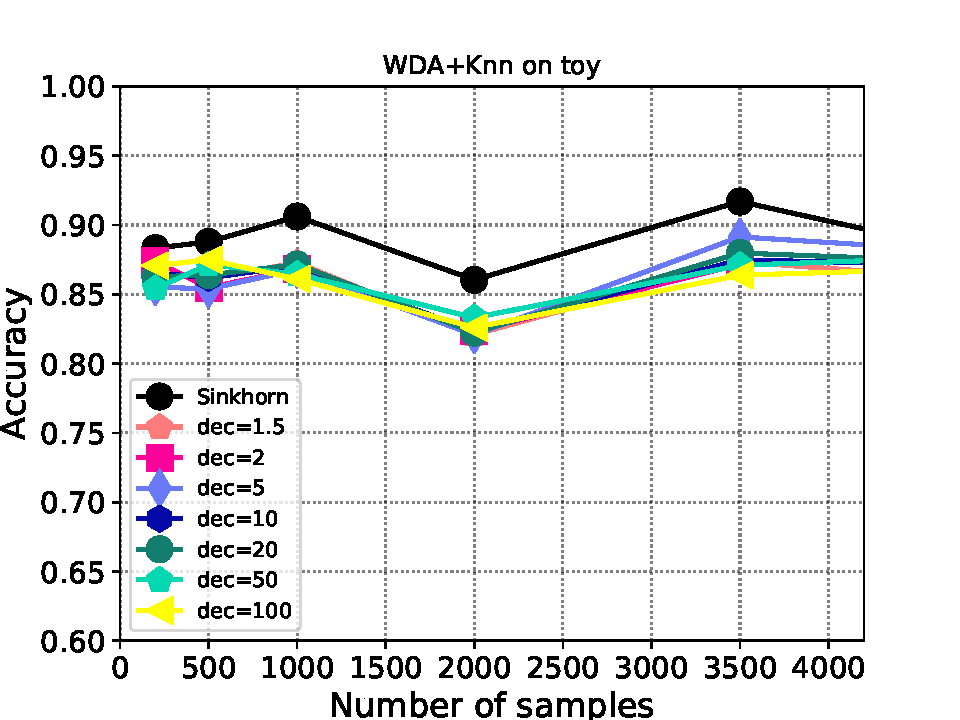
\includegraphics[width=4.cm]{../../figure/wda_accur_toy.pdf}
%	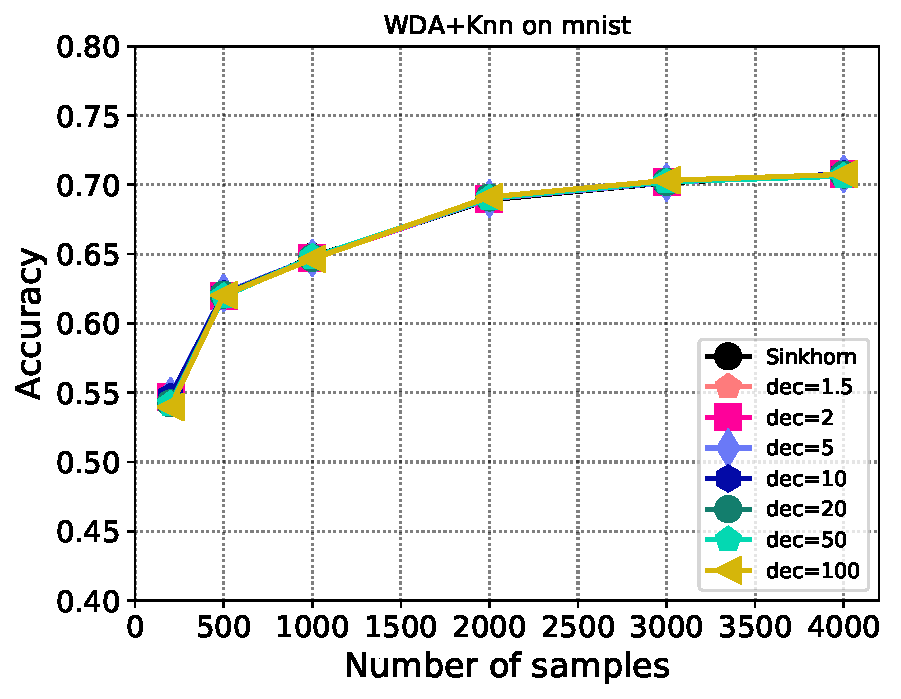
\includegraphics[width=4.cm]{../../figure/wda_accur_mnist.pdf}
	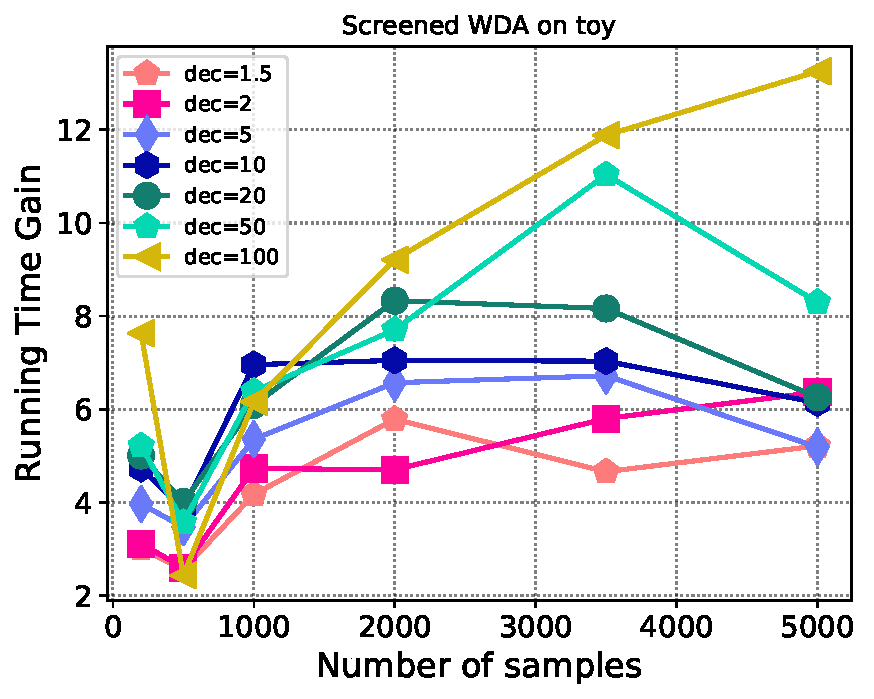
\includegraphics[width=6.cm]{../../figure/wda_gain_toy.pdf}
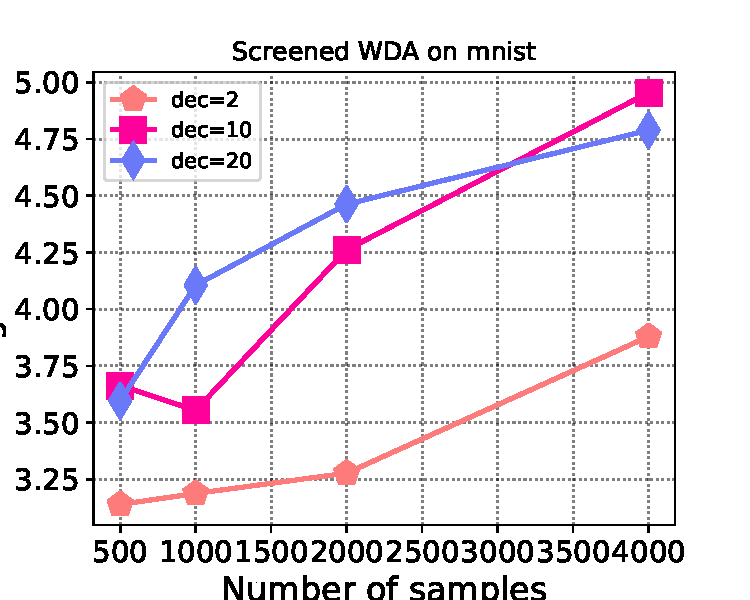
\includegraphics[width=6.cm]{../../figure/wda_gain_mnist.pdf}
	\caption{Wasserstein Discriminant Analysis : running time gain for a toy dataset and for mnist as a function of the number of examples and the data decimation factor in \emph{Screenkhorn}}.
	\label{fig:wda}
\end{figure*}
\begin{figure*}[t]
	\centering

	\includegraphics[width=6.cm]{../../figure/da_gain_toy_regcl1.pdf}
	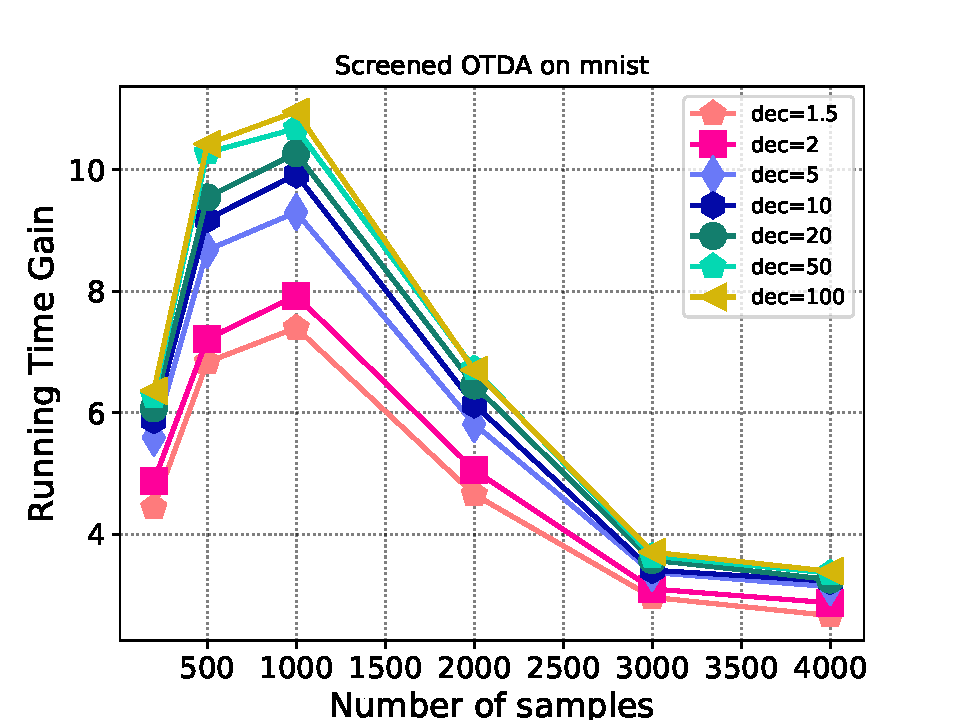
\includegraphics[width=6.cm]{../../figure/da_gain_mnist_regcl1.pdf}
	\caption{OT Domain adaptation : running time gain for a toy dataset and for mnist as a function of the number of examples and the data decimation factor in \emph{Screenkhorn}}.
	\label{fig:otda}
\end{figure*}

For the optimal transport based domain adaptation problem, we have considered the
OTDA with $\ell_{0.5,1}$ group-lasso regularizer that helps in exploiting available labels in the source domain. The problem is solved using an majorization-minimization approach 
for handling the non-convexity of the problem. Hence, at each iteration, a Sinkhorn/Screenkhorn has to be computed. As a domain-adaptation problem, we have
used a MNIST to USPS problem in which features have been extracted from the
feature extractor of an domain adversarial neural networks \cite{ganin2016domain} before full
convergence of the networks (so as to leave room for OT adaptation).



% section numerical_experiments (end)

\section{Conclusion}
The paper proposed a novel efficient approximation of the Sinkhorn divergence
based on a screening strategy. Screening some of the Sinkhorn dual variables
has been made possible by defining a novel constrained dual problem and by 
carefully analyzing its optimality conditions. From the latter, we derived some
sufficient conditions depending on the ground cost matrix, that some dual variables are smaller than a given threshold. Hence, we need just to solve a restricted
dual Sinkhorn problem using an off-the-shelf LBFGS algorithm. We also provided
some theoretical guarantees of the quality of the approximation with respect to
the number of variables that has been screened. Numerical experiments show 
the behaviour of our \emph{Screenkhorn} algorithm and computational time gain it can
achieve when integrated in some complex machine learning pipelines.

% \subsubsection*{Acknowledgments}

% Use unnumbered third level headings for the acknowledgments. All acknowledgments go at the end of the paper. Do not include acknowledgments in the anonymized submission, only in the final paper.

\small
\bibliography{biblio}
\bibliographystyle{chicago}
%well as with those for harvard, apalike, chicago, astron, authordate, and of course natbib.

\newpage
\section{Supplementary material}

\subsection{Proof of Lemma~\ref{lemma_actives_sets}}

Since the objective function $\Psi_{\kappa}$ is convex with respect to $(u,v)$, the set of optima of problem~\eqref{screen-sinkhorn} is non empty.
Introducing two dual variables $\lambda \in \R^n_{+}$ and $\beta \in \R^m_{+}$ for each constraint, the Lagrangian of problem~\eqref{screen-sinkhorn} reads as 
\begin{equation*}
  \mathscr{L}(u,v, \lambda, \beta) = \frac \varepsilon\kappa\inr{\lambda, \mathbf{1}_n} + \varepsilon\kappa\inr{\beta, \mathbf{1}_m} + \mathbf{1}_n^\top B(u,v) \mathbf{1}_m - \inr{\kappa u, \mu} - \inr{\frac v\kappa, \nu} -\inr{\lambda,e^{u}} - \inr{\beta,e^{v}}
\end{equation*}
First order conditions then yield that the Lagrangian multiplicators solutions $\lambda^{*}$ and $\beta^{*}$ satisfy 
\begin{align*}
  &\nabla_u\mathscr{L}(u^{*},v^{*}, \lambda^{*}, \beta^{*})=  e^{u^{*}} \odot(Ke^{v^{*}} - \lambda^{*}) - \kappa\mu = \mathbf 0_n,\\
  & \text{ and } \nabla_v\mathscr{L}(u^{*},v^{*}, \lambda^{*}, \beta^{*})=  e^{v^{*}} \odot(K^\top e^{u^{*}} - \beta) - \frac \nu\kappa = \mathbf 0_m
\end{align*}
which leads to 
\begin{align*}
  &\lambda^{*} = K e^{v^{*}} - \kappa\mu \oslash e^{u^{*}} \text{ and }
  \beta^{*} = K^\top e^{u^{*}} - \nu \oslash \kappa e^{v^{*}}
\end{align*}

For all $i=1, \ldots, n$ we have that $e^{u^{*}_i} \geq \varepsilon\kappa^{-1}$. Further, the condition on the dual variable $\lambda^{*}_i > 0$  ensures that $e^{u^{*}_i} = \varepsilon\kappa^{-1}$ and hence $i \in I^\complement_{\varepsilon,\kappa}$. We have that $\lambda^{*}_i > 0$ is equivalent to $e^{u^{*}_i}r_i(K) e^{v^{*}_j} >  \kappa{\mu_i}$ which  is satisfied when $\varepsilon^2r_i(K) >  \kappa{\mu_i}.$  
In a symmetric way we can prove the same statement for $e^{v^{*}_j}$.

\subsection{Proof of Proposition~\ref{prop:bounds_of_usc_and_vsc}}

We prove only the first statement~\eqref{bound_on_u} and similarly we can prove the second one~\eqref{bound_on_v}.
For all $i\in I_{\varepsilon,\kappa}$, we have $e^{u^{\text{sc}}_i} > \frac \varepsilon\kappa$ or $e^{u^{\text{sc}}_i} = \frac \varepsilon\kappa$. In one hand, if $e^{u^{\text{sc}}_i} > \frac \varepsilon\kappa$ then according to the optimality conditions $\lambda^{\text{sc}}_i = 0,$ which implies $e^{u^{\text{sc}}_i} \sum_{j=1}^m K_{ij} e^{v^{\text{sc}}_j} = \kappa\mu_i$.
In another hand, we have 
\begin{align*}
e^{u^{\text{sc}}_i} \min_{i,j}K_{ij} \sum_{j=1}^m e^{v^{\text{sc}}_j} \leq e^{u^{\text{sc}}_i} \sum_{j=1}^m K_{ij} e^{v^{\text{sc}}_j} = \kappa\mu_i.
\end{align*}
We further observe that $\sum_{j=1}^m e^{v^{\text{sc}}_j} = \sum_{j \in J_{\varepsilon,\kappa}} e^{v^{\text{sc}}_j} + \sum_{j \in J^\complement_{\varepsilon,\kappa}} e^{v^{\text{sc}}_j} \geq \varepsilon\kappa |J_{\varepsilon,\kappa}| + \varepsilon\kappa |J^\complement_{\varepsilon,\kappa}|=\varepsilon\kappa m.$ Then
\begin{equation*}
\max_{i\in I_{\varepsilon,\kappa}} e^{u^{\text{sc}}_i} \leq \frac \varepsilon\kappa \vee \frac{\max_{i\in I_{\varepsilon,\kappa}}\mu_i}{m\varepsilon K_{\min}} \leq \frac \varepsilon\kappa \vee \frac{\max_{i\in I_{\varepsilon,\kappa}}\mu_i}{m\varepsilon K_{\min}}.
\end{equation*}
Analogously, one can obtain for all $j\in J_{\varepsilon,\kappa}$
\begin{equation}
\label{upper_bound_v_potential}
\max_{j\in J_{\varepsilon,\kappa}}e^{v^{\text{sc}}_j} \leq \varepsilon\kappa \vee \frac{\max_{j \in J_{\varepsilon,\kappa}} \nu_j}{n\varepsilon K_{\min}} \leq \varepsilon\kappa \vee \frac{\max_{j \in J_{\varepsilon,\kappa}} \nu_j}{n\varepsilon K_{\min}} .
\end{equation}

Now, since $K_{ij} \leq 1$, we have 
\begin{align*}
e^{u^{\text{sc}}_i} \sum_{j=1}^m e^{v^{\text{sc}}_j} \geq e^{u^{\text{sc}}_i} \sum_{j=1}^m K_{ij}e^{v^{\text{sc}}_j} = \kappa\mu_i.
\end{align*}
Using~\eqref{upper_bound_v_potential}, we get 
\begin{align*}
\sum_{j=1}^m e^{v^{\text{sc}}_j} &= \sum_{j \in J_{\varepsilon,\kappa}} e^{v^{\text{sc}}_j} + \sum_{j \in J^\complement_{\varepsilon,\kappa}} e^{v^{\text{sc}}_j}
\leq \varepsilon\kappa |J^\complement_{\varepsilon,\kappa}| + \varepsilon\kappa \vee \frac{\max_{j\in J_{\varepsilon,\kappa}} \nu_j}{n\varepsilon K_{\min}} |J_{\varepsilon,\kappa}|.
\end{align*}
Therefore,
\begin{align*}
\min_{i \in I_{\varepsilon,\kappa}} e^{u^{\text{sc}}_i}  \geq \frac \varepsilon\kappa \vee \frac{\kappa\min_{I_{\varepsilon,\kappa}}\mu_i}{\varepsilon\kappa (m-m_b) + \varepsilon\kappa \vee \frac{\max_{j\in J_{\varepsilon,\kappa}} \nu_j}{n\varepsilon K_{\min}} m_b}.
\end{align*}

\subsection{Proof of Lemma~\ref{lemma_bounds_on_marginals}}


The optimality condition for $({u}^{\text{sc}}, {v}^{\text{sc}})$ entails 
\begin{align}
\label{i-th-marginal-mu} 
{\mu}^{\text{sc}}_i  &= 
\begin{cases}
e^{u^{\text{sc}}_i} \sum_{j=1}^m K_{ij} e^{v^{\text{sc}}_j}, \text{ if  }i \in I_{\varepsilon,\kappa},\\
\frac \varepsilon\kappa\sum_{j=1}^m K_{ij} e^{v^{\text{sc}}_j}, \text{ if  }i \in I^\complement_{\varepsilon,\kappa}
\end{cases}
=\begin{cases}
\kappa \mu_i, \text{ if  }i \in I_{\varepsilon,\kappa},\\
\frac \varepsilon\kappa\sum_{j=1}^m K_{ij} e^{v^{\text{sc}}_j}, \text{ if  }i \in I^\complement_{\varepsilon,\kappa},
\end{cases}
\end{align}
and 
\begin{align}
\label{i-th-marginal-nu} 
{\nu}^{\text{sc}}_j  &= 
\begin{cases}
e^{v^{\text{sc}}_j} \sum_{i=1}^n K_{ij} e^{u^{\text{sc}}_i}, \text{ if  }j \in J_{\varepsilon,\kappa},\\
\varepsilon\kappa\sum_{i=1}^n K_{ij} e^{u^{\text{sc}}_i}, \text{ if  }j \in J^\complement_{\varepsilon,\kappa}
\end{cases}
=\begin{cases}
\frac{\nu_j}{\kappa}, \text{ if  }j \in J_{\varepsilon,\kappa},\\
\varepsilon\kappa\sum_{i=1}^n K_{ij} e^{u^{\text{sc}}_i}, \text{ if  }j \in J^\complement_{\varepsilon,\kappa}.
\end{cases}
\end{align}

Using inequality~\eqref{bound_on_v}, we obtain 
\begin{align*}
\norm{\mu^{\text{sc}}}_1 &= \sum_{i \in I_{\varepsilon,\kappa}} \mu^{\text{sc}}_i +  \sum_{i \in I^\complement_{\varepsilon,\kappa}}\mu^{\text{sc}}_i\\
& \overset{\eqref{i-th-marginal-mu}}{=} \kappa \norm{\mu_{I_{\varepsilon,\kappa}}^{\text{sc}}}_1 + \frac \varepsilon\kappa \sum_{i \in I^\complement}\Big( \sum_{j \in J_{\varepsilon,\kappa}} K_{ij} e^{v^{\text{sc}}_j} + \varepsilon\kappa \sum_{j\in J^\complement_{\varepsilon,\kappa}}K_{ij}\Big)\\
& \overset{\eqref{bound_on_v}}{\leq} \kappa \norm{\mu_{I_{\varepsilon,\kappa}}^{\text{sc}}}_1 + (n-n_b) \Big(\frac{m_b\max_{j \in J_{\varepsilon,\kappa}} \nu_j}{n\kappa K_{\min}} + (m-m_b)\varepsilon^2 \Big).
\end{align*}
Again by left-hand-side of inequaltiy~\eqref{bound_on_v}, we arrive at 
\begin{align*}
\norm{\mu^{\text{sc}}}_1 %&= \sum_{i \in I_{\varepsilon,\kappa}} \mu^{\text{sc}}_i +  \sum_{i \in I^\complement_{\varepsilon,\kappa}}\mu^{\text{sc}}_i\\
%& \overset{\eqref{i-th-marginal-mu}}{=} \kappa \norm{\mu_{I_{\varepsilon,\kappa}}^{\text{sc}}}_1 + \frac \varepsilon\kappa \sum_{i \in I^\complement}\Big( \sum_{j \in J_{\varepsilon,\kappa}} K_{ij} e^{v^{\text{sc}}_j} + \varepsilon\kappa \sum_{j\in J^\complement_{\varepsilon,\kappa}}K_{ij}\Big)\\
& \overset{}{\geq} \kappa \norm{\mu_{I_{\varepsilon,\kappa}}^{\text{sc}}}_1 + (n -n_b) \Big(\frac{mm_b\varepsilon^2 K_{\min}^2 \min_{j\in J_{\varepsilon, \kappa}} \nu_j}{ (n-n_b)m\kappa \varepsilon^2 K_{\min} + n_b\kappa^2 \max_{i\in I_{\varepsilon,\kappa}}\mu_i }+ (m-m_b)\varepsilon^2K_{\min}\Big),
\end{align*}
which gives the claimed result.
Similarly, we can prove the same statement for $\norm{\nu^{\text{sc}}}_1$.

\subsection{Proof of Proposition~\ref{proposition_error_in_marginals}}

We define the distance function $\varrho: \R_+ \times \R_+ \mapsto [0, \infty]$ by $\varrho(a,b) = b - a + a \log(\frac ab).$
While $\varrho$ is not a metric, it is easy to see that $\varrho$ is not nonnegative and satisfies $\varrho(a,b) =0$ iff $a=b$.
The violations are computed through the following function: 
\begin{equation*}
	d_{\varrho}(\gamma,\beta) = \sum_{i=1}^n \varrho(\gamma_i,\beta_i), \text{ for } \gamma, \beta \in \R^n_+.
\end{equation*}
Note that if $\gamma,\beta$ are two vectors of positive entries, $d_{\varrho}(\gamma,\beta)$ will return some measurement on how far they are from each other. The next Lemma is from~\cite{khalilabid2018} (see Lemma 7 herein).
\begin{lemma}
\label{lem:pinsker}
For any $\gamma, \beta \in \R^n_+$, the following generalized Pinsker inequality holds 
\begin{align*}
\norm{\gamma - \beta}_1 \leq \sqrt{7 (\norm{\gamma}_1\wedge \norm{\beta}_1)d_{\varrho}(\gamma,\beta)}
\end{align*}
\end{lemma}
By~\eqref{i-th-marginal-mu}, we have
\begin{align*}
d_\varrho({\mu} ,{\mu}^{\text{sc}}) &= \sum_{i=1}^n  {\mu}^{\text{sc}}_i - {\mu}_i + {\mu}_i  \log\Big(\frac{{\mu}_i}{{\mu}^{\text{sc}}_i }\Big)\\
&= \sum_{i\in I_{\varepsilon,\kappa}} (\kappa-1)\mu_i - \mu_i\log(\kappa) + \sum_{i\in I^\complement_{\varepsilon,\kappa}}\frac \varepsilon\kappa\sum_{j=1}^m K_{ij} e^{v^{\text{sc}}_j} - \mu_i + \mu_i \log\Big(\frac{\mu_i}{\frac \varepsilon\kappa\sum_{j=1}^m K_{ij} e^{v^{\text{sc}}_j}}\Big)\\
&= \sum_{i\in I_{\varepsilon,\kappa}} (\kappa-\log(\kappa)-1)\mu_i  + \sum_{i\in I^\complement_{\varepsilon,\kappa}}\frac \varepsilon\kappa\sum_{j=1}^m K_{ij} e^{v^{\text{sc}}_j} - \mu_i + \mu_i \log\Big(\frac{\mu_i}{\frac \varepsilon\kappa\sum_{j=1}^m K_{ij} e^{v^{\text{sc}}_j}}\Big).
% &\leq  \sum_{i\in I^\complement_{\varepsilon,\kappa}}\frac \varepsilon\kappa\sum_{j=1}^m K_{ij} e^{v^{\text{sc}}_j} - \mu_i + \mu_i \log\Big(\frac{\mu_i}{\frac \varepsilon\kappa\sum_{j=1}^m K_{ij} e^{v^{\text{sc}}_j}}\Big)
\end{align*}
Now by~\eqref{bound_on_v}, we have in one hand 
\begin{align*}
\sum_{i\in I^\complement_{\varepsilon,\kappa}}\frac \varepsilon\kappa\sum_{j=1}^m K_{ij} e^{v^{\text{sc}}_j}&= \sum_{i\in I^\complement_{\varepsilon,\kappa}}\frac \varepsilon\kappa \Big(\sum_{j\in J_{\varepsilon,\kappa}}K_{ij} e^{v^{\text{sc}}_j} + \varepsilon \kappa\sum_{j\in J^\complement_{\varepsilon,\kappa}}K_{ij}\Big)\\
&\leq \sum_{i\in I^\complement_{\varepsilon,\kappa}}\frac \varepsilon\kappa \Big(m_b \max_{i,j}K_{ij}\frac{\max_{j \in J_{\varepsilon,\kappa}} \nu_j}{n\varepsilon K_{\min}} + (m - m_b)\varepsilon\kappa\max_{i,j}K_{ij}\Big) \\
&\leq (n-n_b)\Big(\frac{m_b\max_{j} \nu_j}{n\kappa K_{\min}} + (m- m_b) \varepsilon^2\Big).
\end{align*}
On the other hand, we get
\begin{align*}
\frac \varepsilon\kappa\sum_{j=1}^m K_{ij} e^{v^{\text{sc}}_j}&=\frac \varepsilon\kappa \Big(\sum_{j\in J_{\varepsilon,\kappa}}K_{ij} e^{v^{\text{sc}}_j} + \varepsilon \kappa\sum_{j\in J^\complement_{\varepsilon,\kappa}}K_{ij}\Big)\\
&\geq m_bK_{\min} \frac{m\varepsilon^2K_{\min}\min_{j \in J_{\varepsilon,\kappa}}\nu_j}{\kappa((n-n_b)m\varepsilon^2K_{\min} + m\varepsilon^2K_{\min} + n_b\kappa\max_{i\in I_{\varepsilon,\kappa}}\mu_i)}\\
&\qquad +\varepsilon^2 (m- m_b) K_{\min}\\
&\geq \frac{mm_b\varepsilon^2(K_{\min})^2\min_{j \in J_{\varepsilon,\kappa}}\nu_j}{\kappa((n-n_b)m\varepsilon^2K_{\min}+ m\varepsilon^2K_{\min} + n_b\kappa\max_{i\in I_{\varepsilon,\kappa}}\mu_i)}\\
&\qquad +\varepsilon^2 (m- m_b) K_{\min}\\
&\geq \frac{mm_b\varepsilon^2K_{\min}^2\min_{j \in J_{\varepsilon,\kappa}}\nu_j}{\kappa((n-n_b)m\varepsilon^2K_{\min}+ m\varepsilon^2K_{\min} + n_b\kappa\max_{i\in I_{\varepsilon,\kappa}}\mu_i)}.
\end{align*}
Then 
\begin{align*}
\frac{1}{\frac \varepsilon\kappa\sum_{j=1}^m K_{ij} e^{v^{\text{sc}}_j}} &\leq \frac{\kappa((n-n_b)m\varepsilon^2K_{\min}+ m\varepsilon^2K_{\min} + n_b\kappa\max_{i\in I_{\varepsilon,\kappa}}\mu_i)}{mm_b\varepsilon^2 K_{\min}^2\min_{j \in J_{\varepsilon,\kappa}}\nu_j}\\
&\leq \frac{\kappa(n-n_b+ 1)}{m_bK_{\min}\min_{j \in J_{\varepsilon,\kappa}}\nu_j} + \frac{n_b\kappa^2\max_{i\in I_{\varepsilon,\kappa}}\mu_i}{mm_b\varepsilon^2K_{\min}^2\min_{j \in J_{\varepsilon,\kappa}}\nu_j}.
\end{align*}
It entails 
\begin{align*}
&\sum_{i\in I^\complement_{\varepsilon,\kappa}}\frac \varepsilon\kappa\sum_{j=1}^m K_{ij} e^{v^{\text{sc}}_j} - \mu_i + \mu_i \log\Big(\frac{\mu_i}{\frac \varepsilon\kappa\sum_{j=1}^m K_{ij} e^{v^{\text{sc}}_j}}\Big)\\
&\leq (n-n_b)\bigg(\frac{m_b}{n\kappa\min_{i,j} K_{ij}} + (m- m_b) \varepsilon^2 - \min_{i}\mu_i\\
&\qquad + \max_{i}\mu_i\log\Big(\frac{\kappa(n-n_b+ 1)\max_{i}\mu_i}{m_bK_{\min}\min_{j \in J_{\varepsilon,\kappa}}\nu_j} + \frac{n_b\kappa^2(\max_{i}\mu_i)^2}{mm_b\varepsilon^2 K_{\min}^2\min_{j \in J_{\varepsilon,\kappa}}\nu_j}\Big)
\bigg).
\end{align*}
Therefore
\begin{align*}
d_\varrho({\mu},{\mu}^{\text{sc}}) &\leq n_b(\kappa-\log(\kappa)-1)\max_{i} \mu_i + (n-n_b)\bigg(\frac{m_b\max_{j}\nu_j}{n\kappa\min_{i,j} K_{ij}} + (m- m_b) \varepsilon^2 - \min_{i}\mu_i\\
&\qquad + \max_{i} \mu_i\log\Big(\frac{\kappa(n-n_b+ 1)\max_{i} \mu_i}{m_bK_{\min}\min_{j \in J_{\varepsilon,\kappa}}\nu_j} + \frac{n_b\kappa^2(\max_{i} \mu_i)^2}{mm_b\varepsilon^2 K_{\min}^2\min_{j \in J_{\varepsilon,\kappa}}\nu_j}\Big).
\end{align*}
Finally, by Lemma~\ref{lem:pinsker} we obtain
\begin{align*}
\norm{{\mu} -{\mu}^{\text{sc}}}^2_1 \leq & n_b(\kappa-\log(\kappa)-1)\max_{i} \mu_i + 7(n-n_b)\bigg(\frac{m_b\max_{j}\nu_j}{n\kappa\min_{i,j} K_{ij}} + (m- m_b) \varepsilon^2 - \min_{i}\mu_i\\
&+ \max_{i} \mu_i\log\Big(\frac{\kappa(n-n_b+ 1)\max_{i} \mu_i}{m_bK_{\min}\min_{j \in J_{\varepsilon,\kappa}}\nu_j} + \frac{n_b\kappa^2(\max_{i} \mu_i)^2}{mm_b\varepsilon^2K_{\min}^2\min_{j \in J_{\varepsilon,\kappa}}\nu_j}\Big).%\bigg\}^{1/2}
\end{align*}
Proof of the upper bound for $\norm{\nu - {\nu}^{\text{sc}}}^2_1$ follows the same lines as above.



\subsection{Additional experimental results}

\end{document}